\section{Source Files}
This appendix briefly introduces all source files of this XG-PON module for NS-3.

\begin{enumerate}
 \item pon-channel.h/.cc: source code for {\color{red} PonChannel}. 
PonChannel has implemented how to send one upstream frame from one ONU to the OLT 
and how to broadcast one downstream frame from the OLT to all ONUs. 
It is one abstract class and its subclass should manage the OLT and all ONUs 
attached on the channel, especially the propagation delay between the OLT and each ONU. 
When subclass instantiates PonChannel, each ONU should have one unique index in the PonChannel and this index can be used to get its corresponding propagation delay.

 \item pon-frame.h: source code for {\color{red} PonFrame}. 
PonFrame is one abstract class with the interfaces for (de)serialization.

 \item pon-net-device.h/.cc: source code for {\color{red} PonNetDevice}. 
PonNetDevice is inherited from NetDevice of NS-3. 
It defines one abstract function "ReceivePonFrameFromChannel" that 
should be implemented by its subclass for handling frames received from PonChannel. 
It also maintains the index of this device on the PonChannel. 
This index is useful to ONU only for getting its propagation delay.
\\
{\color{blue} This group of files are used to model a general 
TDMA-based Passive Optical Network. EPON could also be implemented 
through instantiating these classes.}
\vspace{0.3in}



 \item xgpon-burst-profile.h/.cc: source code for {\color{red} XgponBurstProfile}. 
XgponBurstProfile implements the burst profile used by one ONU to produce one upstream burst. 
It specifies the physical layer overhead (the length of preamble and delimiter) and 
whether FEC is used for this burst. When the OLT assigns one upstream transmission opportunity to one ONU, 
it also notifies the ONU about the burst profile to be used. Thus, one ONU may use different 
burst profile for different bursts at different times. 
The OLT may make decision based on channel quality and the kind of payload, etc.

 \item xgpon-key.h/.cc: source code for {\color{red} XgponKey}. XgponKey is used to carry out encryption. 
It is just one stub class to be instantiated in the future if key management needs to be studied.

 \item xgpon-link-info.h/.cc: source code for {\color{red} XgponLinkInfo}. 
XgponLinkInfo is used to maintain the information of one ONU, such as the keys and 
burst profiles negotiated between the OLT and this ONU. It also includes 
the corresponding equalization delay of this ONU for avoiding collision in upstream direction. 
XgponLinkInfo also maintains one list of PLOAM messages to be sent to the OLT (at ONU side) 
or the corresponding ONU (at OLT side). It also includes many other state information 
to achieve various purposes through PLOAM messages, the header of downstream frame, 
the header of upstream burst, and the header of XGEM frame.
\\
{\color{blue} This group of files are used to represent the information of one ONU, 
especially keys, burst profiles, PLOAM messages, and equalization delay. XgponLinkInfo 
will be managed by XgponOltPloamEngine and XgponOnuPloamEngine so that other engines 
of XgponNetDevice can get the corresponding information.}
\vspace{0.3in}




 \item xgpon-xgtc-ploam.h/.cc: source code for {\color{red} XgponXgtcPloam}.XgponXgtcPloam is used to
represent one PLOAM message exchanged between OLT and ONU. Since PLOAM messages need to 
be allocated and released dynamically during simulation, the new and delete operators of XgponXgtcPloam 
are overridden and a pool is maintained for reducing the cost of the expensive "malloc" operations.

 \item xgpon-xgem-header.h/.cc: source code for {\color{red} XgponXgemHeader}. XgponXgemHeader is 
the header of XGEM frame exchanged between OLT and ONU. It is one member variable of the following
XgponXgemFrame.

 \item xgpon-xgem-frame.h/.cc: source code for {\color{red} XgponXgemFrame}. 
XgponXgemFrame is used to encapsulate SDU from upper layers. Except one XgponXgemHeader 
and the potential SDU, it also has one member variable used to specify the type of this XGEM frame 
(normal frame, idle frame, or short idle frame). Since huge amount of XGEM frames
need to be allocated and released dynamically, its new and delete
operators are also overridden and a pool is maintained for
reducing the cost of the expensive "malloc" operations.
\vspace{0.1in}

 \item xgpon-ds-frame.h/.cc: source code for {\color{red} XgponDsFrame}. XgponDsFrame is one subclass of PonFrame for XG-PON.
 It is designed to represent one downstream frame broadcasted from OLT to ONUs. It mainly contains two member variables,
 one for physical layer header (XgponPsbd) and the other for XGTC layer downstream frame (XgponXgtcDsFrame).
 For saving CPU used to allocate and release this structure, its new and delete operators are also overridden
 and a pool is maintained for reducing the cost of the expensive
 "malloc" operations.

 \item xgpon-psbd.h/.cc: source code for {\color{red} XgponPsbd}. XgponPsbd is the physical layer header of the downstream frame of XG-PON (XgponDsFrame).

 \item xgpon-xgtc-ds-frame.h/.cc: source code for {\color{red} XgponXgtcDsFrame}. 
XgponXgtcDsFrame is the downstream frame observed by XGTC layer. It mainly includes one XGTC layer header 
(XgponXgtcDsHeader) and a bunch of XGEM frames. To allow hundreds of ONUs to process one XgponXgtcDsFrame 
quickly, we separate the broadcasted XGEM frames that must be processed by all ONUs and the uni-casted ones. 
Considering that one XgponXgtcDsFrame may contain the traffic of just a few ONUs, most of ONUs need not 
parse these uni-casted XGEM frames for extracting their own traffic. Thus, a bitmap is also added into XgponXgtcDsFrame 
to indicate the ONUs whose traffic are within this frame.

 \item xgpon-xgtc-ds-header.h/.cc: source code for {\color{red} XgponXgtcDsHeader}. 
XgponXgtcDsHeader is the XGTC layer header of a downstream frame (XgponXgtcDsFrame). 
It contains a list of PLOAM messages (XgponXgtcPloam) to be sent to ONUs and the 
following XgponXgtcBwmap used to instruct ONUs how to share the upstream wavelength.

 \item xgpon-xgtc-bwmap.h/.cc: source code for {\color{red} XgponXgtcBwmap}. XgponXgtcBwmap is produced by the OLT and broadcasted to all ONUs in the header of the XGTC downstream frame (XgponXgtcDsHeader). It is used to instruct ONUs how to share the upstream wavelength in a TDMA-like manner.
 It includes a list of the following XgponXgtcBwAllocation. For saving CPU used to allocate and release this structure, its new and delete operators are also overridden and a pool is maintained for reducing the cost of the expensive "malloc"
 operations.

 \item xgpon-xgtc-bw-allocation.h/.cc: source code for {\color{red} XgponXgtcBwAllocation}. In XgponXgtcBwmap, 
there is one XgponXgtcBwAllocation for each T-CONT scheduled in the corresponding upstream frame. 
XgponXgtcBwAllocation is used to specify when one ONU should send the upstream traffic of this T-CONT, 
how many bytes it can send, and whether it can send one queue occupancy report. The XgponXgtcBwAllocation of 
the same ONU will form one upstream burst. For the first XgponXgtcBwAllocation of the same burst, 
it also specifies the burst profile used by the corresponding upstream burst and whether the ONU can 
send one PLOAM message to the OLT.  For saving CPU used to allocate and release this structure, 
its new and delete operators are also overridden and a pool is maintained for reducing the cost of 
the expensive "malloc" operations.
\vspace{0.1in}

 \item xgpon-us-burst.h/.cc: source code for {\color{red} XgponUsBurst}. XgponUsBurst is one subclass 
of PonFrame for XG-PON. It is designed to represent one upstream burst that one ONU sends to the OLT 
in upstream direction. It mainly contains two member variables, one for physical layer header (XgponPsbu) 
and the other for XGTC layer upstream burst (XgponXgtcUsBurst). For saving CPU used to allocate and 
release this structure, its new and delete operators are also overridden and a pool is maintained for 
reducing the cost of the expensive "malloc" operations.

 \item xgpon-psbu.h/.cc: source code for {\color{red} XgponPsbu}. XgponPsbu is the physical layer header 
of the upstream burst of XG-PON (XgponUsBurst). It contains the preamble and delimiter. 
Their length is determined by the burst profile used for this burst. And the burst profile is 
selected by the OLT and specified in the corresponding XgponXgtcBwmap.

 \item xgpon-xgtc-us-burst.h/.cc: source code for {\color{red} XgponXgtcUsBurst}. 
XgponXgtcUsBurst is the upstream burst observed by XGTC layer. It mainly includes 
one XGTC layer header (XgponXgtcUsHeader), a trailer, and a bunch of the following 
XgponXgtcUsAllocation (one for each T-CONT).

 \item xgpon-xgtc-us-header.h/.cc: source code for {\color{red} XgponXgtcUsHeader}. XgponXgtcUsHeader 
is the XGTC layer header of an upstream burst (XgponXgtcUsBurst). If scheduled by the OLT, 
one PLOAM message can also be sent to the OLT within this header.

 \item xgpon-xgtc-us-allocation.h/.cc: source code for {\color{red} XgponXgtcUsAllocation}. 
XgponXgtcUsAllocation is designed to represent the traffic of one T-CONT to be transmitted 
in the upstream burst. It mainly contains a bunch of XGEM frames. If scheduled by the OLT 
through XgponXgtcBwmap, one queue occupancy report (XgponXgtcDbru) is also transmitted in 
XgponXgtcUsAllocation. For saving CPU used to allocate and release this structure, 
its new and delete operators are also overridden and a pool is maintained for reducing 
the cost of the expensive "malloc" operations.

 \item xgpon-xgtc-dbru.h/.cc: source code for {\color{red} XgponXgtcDbru}. 
XgponXgtcDbru is used to represent one queue occupancy report of one T-CONT.
\\
{\color{blue} This group of files are used to represent the
information communicated between the OLT and ONU. For all of these
classes, they should support the (de)serialization. Since the
current simulation is carried out in the same thread of the same
computer and it could be quite complex, we have not fully
implemented this feature. However, "GetSerializedSize()" has been
implemented for all so that we can compose the downstream frame
and upstream burst with considering their length constraints. In
many of these classes, some error detection/correction coding
schemes are used to be robust to transmission error. In current
phase, these algorithms are not implemented and we assume that
these structures are correct. In the future, transmission errors
might be simulated through discarding one whole frame/burst.
Furthermore, in many of these classes, some meta-data member
variables are added to facilitate (de)serialization and maintain
some time-related information (creation time, receiving time,
etc.). For instance, XgponXgtcBwmap maintains its creation time.
The OLT uses this information, the logic one-way-delay of the
channel, and the time that a upstream burst is received, to
associate this upstream burst to its corresponding XgponXgtcBwmap.
Figure \ref{fig_xgpon_frame_files} summarizes how these classes
are used to represent the frame/burst transmitted in XG-PON. }

\begin{figure}[!htbp]
\begin{center}
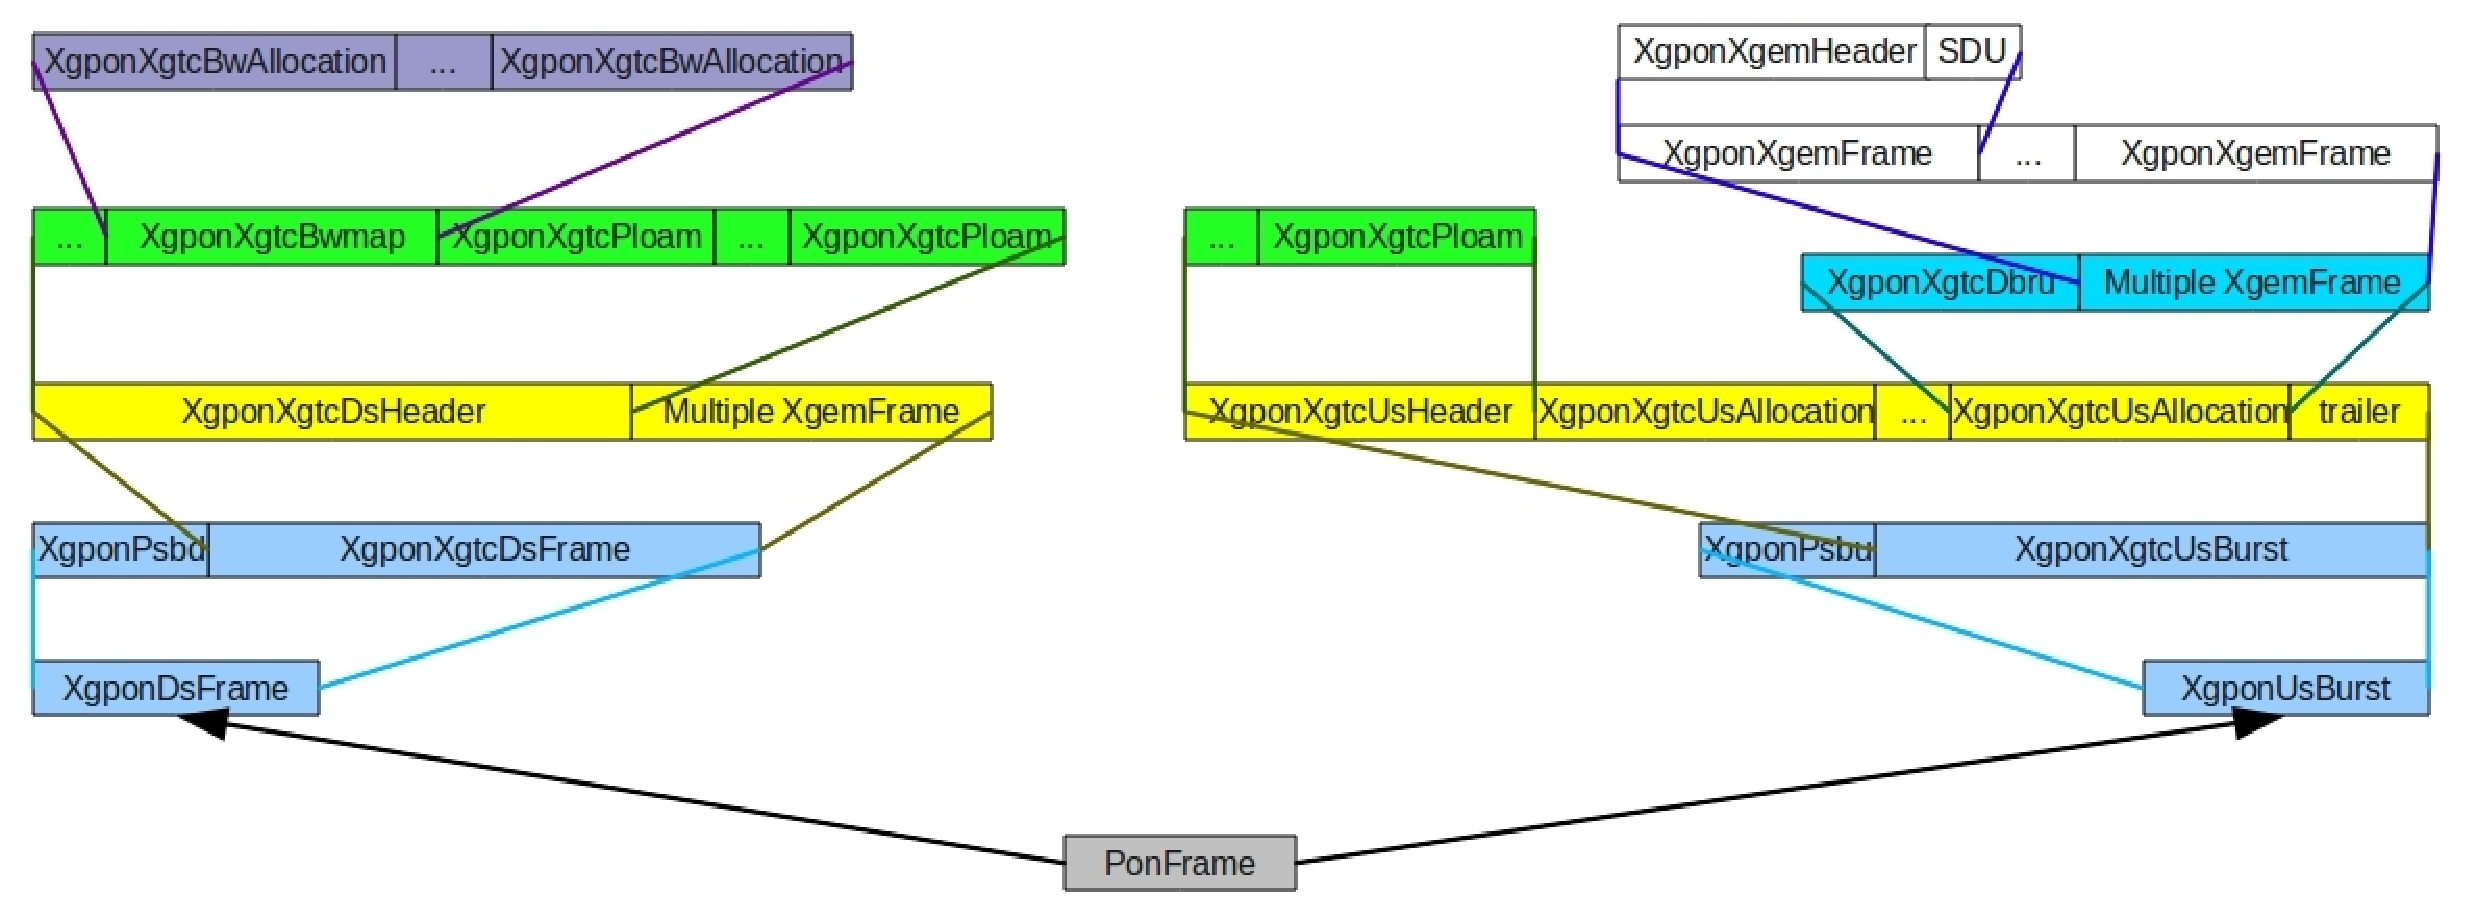
\includegraphics[width=0.99\textwidth]{images/xgponframefiles}
\end{center}
\vspace{-0.1in}
\caption{Classes for frame/burst of XG-PON}
\label{fig_xgpon_frame_files}
\end{figure}

\vspace{0.3in}



 \item xgpon-qos-parameters.h/.cc: source code for {\color{red} XgponQosParameters}. XgponQosParameters is used to 
hold the Qos parameters of one XGEM Port or T-CONT (aggregated from its XGEM Ports) that XG-PON should satisfy. 
Its content follows XG-PON standard, such as fixed bandwidth, assured bandwidth, etc.

 \item xgpon-connection.h/.cc: source code for {\color{red} XgponConnection}. XgponConnection is used to represent 
one XGEM Port of XG-PON. It is one abstract class with basic information (the direction, Broadcast or Uni-cast, 
XGEM Port-Id, Alloc-Id for upstream XGEM Port, ONU-ID that this XGEM Port belongs to, and upper layer address of 
the computer whose traffic this XGEM Port will carry) and its QoS parameters should be satisfied by XG-PON. 
XgponConnectionReceiver is the subclass for the receiver and XgponConnectionSender is the subclass for the sender. 
Thus, for one upstream XGEM Port, there is one XgponConnectionSender at ONU and one corresponding XgponConnectionReceiver 
at OLT. For the downstream XGEM Port, there is one XgponConnectionSender at OLT and one corresponding XgponConnectionReceiver 
at ONU. The QoS parameters at the sender and the receiver must be identical.

 \item xgpon-connection-receiver.h/.cc: source code for {\color{red} XgponConnectionReceiver}. As the subclass of XgponConnection 
for the receiver, XgponConnectionReceiver is quite simple. It mainly holds the segments that have been received to carry out 
reassemble in the future. Note that, for upstream traffic, reassemble is carried out by the OLT per T-CONT.

 \item xgpon-connection-sender.h/.cc: source code for {\color{red} XgponConnectionSender}. XgponConnectionSender 
is the XGEM Port instance at the sender. It has one queue (XgponQueue) to buffer the traffic to be transmitted 
on XG-PON and a list of service records (XgponServiceRecord) that could be used for scheduling purposes. 
It is also responsible to receive the SDU (put it into the queue), get the packet to be transmitted on XG-PON 
(fragmentation needs to be considered), maintain its serving history (a list of XgponServiceRecord), 
and return the occupancy of its queue.

 \item xgpon-service-record.h/.cc: source code for {\color{red} XgponServiceRecord}. XgponServiceRecord is used to 
store the event that one XGEM Port is served. It records the time that the traffic of this XGEM Port are transmitted 
and the amount of bytes transmitted through XG-PON. For saving CPU used to allocate and release this structure, 
its new and delete operators are also overridden and a pool is maintained for reducing the cost of the expensive "malloc" operations.

 \item xgpon-queue.h/.cc: source code for {\color{red} XgponQueue}. XgponQueue is used for each XGEM Port at the sender. 
It is used to hold the traffic to be transmitted through XG-PON. Instead of Queue from NS-3, XgponQueue is added for 
three reasons. First, fragmentation need to be considered and it should hold the remaining part of one fragmented 
SDU and send the remaining part immediately once this XGEM Port is served again. Second, some variables in 
ns3::Queue are private and we cannot update them. Third, when SDU is encapsulated into XGEM frame, padding 
must be carried out for word-alignment. Thus, queue occupancy must be updated accordingly. 
Instead of calculating queue occupancy (visiting each packet in the queue) when needed, 
this value is maintained when packet is enqueued/dequeued, two calculations are necessary for each packet, 
and CPU can be saved. Note that XgponQueue is one abstract class and its subclass 
is responsible to manage packets in the queue and implement some queue discipline.

 \item xgpon-fifo-queue.h/.cc: source code for {\color{red} XgponFifoQueue}. XgponFifoQueue is one subclass 
of XgponQueue and it follows the principles of FIFO (First In, First Out).
\vspace{0.1in}


 \item xgpon-tcont.h/.cc: source code for {\color{red} XgponTcont}. XgponTcont is used to represent 
one T-CONT (Note that one T-CONT might have multiple upstream XGEM Ports) of XG-PON. It is one abstract class 
with basic information (Alloc-Id, ONU-ID that this T-CONT belongs to). XgponTcontOlt is the subclass used by 
the OLT and XgponTcontOnu is the subclass used by ONU. In addition, XgponTcont also holds a list of XgponXgtcDbru 
(the history of queue occupancy reports) and a list of XgponXgtcBwAllocation (the serving history) 
related with this T-CONT. These information could be used by the OLT to deduce how many data of this T-CONT 
is still waiting at ONU to be served.

 \item xgpon-tcont-olt.h/.cc: source code for {\color{red} XgponTcontOlt}. XgponTcontOlt is the T-CONT instance 
at the OLT. It has a list of XgponConnectionReceiver that are used to calculate its aggregated QoS parameters. 
It is responsible to carry out reassemble, receive queue occupancy report from ONU, maintain its serving history 
and queue occupancy reports, and calculate the amount of data at ONU that still needs to be served. 
When there is no queue occupancy reports from ONU, it is also responsible to tell the OLT whether to 
poll the ONU for the status of this T-CONT.

 \item xgpon-tcont-onu.h/.cc: source code for {\color{red} XgponTcontOnu}. XgponTcontOnu is the T-CONT instance 
at ONU. It has a list of XgponConnectionSender that belong to this T-CONT. It is responsible to maintain these connections, 
generate queue occupancy report, and maintain the serving history (a list of XgponXgtcBwAllocation from the OLT). 
Since the OLT just assigns the upstream bandwidth to T-CONTs, XgponTcontOnu has one upstream scheduler (XgponOnuUsScheduler) 
used to schedule traffic of the connections that belong to the same T-CONT. Through putting one upstream scheduler 
into XgponTcontOnu, we can use different upstream schedulers for different T-CONTs.

 \item xgpon-onu-us-scheduler.h/.cc: source code for {\color{red} XgponOnuUsScheduler}. XgponOnuUsScheduler is used to 
schedule traffic of the connections that belong to the same T-CONT. When one upstream burst need to be produced, 
XgponOnuUsScheduler is used by ONU to determine the traffic to be put into this burst. The main interface is "SelectConnToServe", 
a virtual function that its subclass must be implement to determine the connection to be served and 
the amount of data to be transmitted.

 \item xgpon-onu-us-scheduler-round-robin.h/.cc: source code for {\color{red} XgponOnuUsSchedulerRoundRobin}. 
XgponOnuUsSchedulerRoundRobin is one subclass of XgponOnuUsScheduler that schedules the upstream connections of 
the same T-CONT in round-robin manner with considering their queue occupancy.
\\
{\color{blue} This group of files are used to represent XGEM Port and T-CONT in XG-PON. At the sender, there is 
one queue for each XGEM Port. Fragmentation and reassemble are considered in these classes. Qos parameters and 
serving history are also maintained in these classes. }
\vspace{0.3in}









 \item xgpon-channel.h/.cc: source code for {\color{red} XgponChannel}. XgponChannel is a subclass of PonChannel for XG-PON. 
It maintains the logic one-way-delay for the whole XG-PON network, which should be set based on the largest propagation 
delay among all ONUs and various processing delays. In XG-PON, all nodes (OLT and ONUs) have a consistent view of this value. 
Correspondingly, each ONU has one equalization delay that is related with the logic one-way-delay and its 
own propagation delay (between this ONU and the OLT).

 \item xgpon-phy.h/.cc: source code of {\color{red} XgponPhy}. XgponPhy contains the physical layer parameters of 
one XG-PON network and provides several common routines. These parameters can be configured through NS-3 attribute system. 
Through changing these parameters, we could simulate GPON approximately.

 \item xgpon-net-device.h/.cc: source code for {\color{red} XgponNetDevice}. XgponNetDevice is a subclass of PonNetDevice 
that implements the common functions for both OLT and ONU. It implements "Send" and "SendFrom" inherited from NetDevice 
for accepting packets from upper layers. However, these functions just trace these events and the main jobs are done 
by "DoSend" and "DoSendFrom" that will be instantiated by XgponOnuNetDevice and XgponOltNetDevice. XgponNetDevice also 
provides functions to other components for sending SDU to upper layers and supporting Pcap and Ascii tracing. 
It also maintains a per-device statistics, such as the amount of data received from upper layer, dropped due to 
buffer overflow, etc. It also has one instance of XgponPhy so that the engines of XgponOltNetDevice/XgponOnuNetDevice 
can get to know physical layer parameters used in simulation.

 \item xgpon-olt-net-device.h/.cc: source code for {\color{red} XgponOltNetDevice}. XgponOltNetDevice is a subclass 
of XgponNetDevice for the OLT. It has a bunch of engines that implement various functions of the XGTC layer for the OLT. 
These engines will be introduced below. XgponOltNetDevice has implemented "ReceivePonFrameFromChannel" for processing 
the upstream bursts from ONUs with its engines. It also has implemented "DoSend" and "DoSendFrom" to put the packets 
from the upper layers to their corresponding queues. When this class is initiated at the beginning of the simulation, 
"SendDownstreamFrameToChannelPeriodically" is called to periodically (125 micro-second) generate a downstream frame with 
its engines and pass the frame to XgponChannel for broadcasting to all ONUs.

 \item xgpon-onu-net-device.h/.cc: source code for {\color{red} XgponOnuNetDevice}. XgponOnuNetDevice is a subclass 
of XgponNetDevice for ONU. It has a bunch of engines that implement various functions of the XGTC layer for ONU. 
XgponOnuNetDevice has implemented "ReceivePonFrameFromChannel" for processing the downstream frames from the OLT with its engines. 
It also has implemented "DoSend" and "DoSendFrom" to put the packets from the upper layers to their corresponding queues. 
XgponOnuNetDevice also provides "ProduceAndTransmitUsBurst" in which one upstream burst is produced with its engines 
and pass to XgponChannel for sending to the OLT. This function is used when ONU processes XgponXgtcBwmap and schedules 
to produce the burst assigned by the OLT.
\\
{\color{blue} This group of files are used to implement XG-PON through instantiating PonNetDevice and PonChannel. 
Within XgponOltNetDevice, their engines need to call each other's functions quite frequently. Although we can 
decouple these engines through adding functions into XgponOltNetDevice (these functions will simply delegate 
the tasks to the corresponding engines), these engines are tightly coupled and too many functions need to be added. 
Thus, we let each engine have one reference of XgponOltNetDevice and the engine can access other engines through 
XgponOltNetDevice. For XgponOnuNetDevice, the situation is similar and we handle in the same way.}
\vspace{0.3in}




 \item xgpon-olt-engine.h/.cc: source code for {\color{red} XgponOltEngine}. XgponOltEngine is the base class of the following engines 
used by XgponOltNetDevice. Through inheriting from XgponOltEngine, each engine will have one reference of XgponOltNetDevice, 
which can be used to access other related engines.

 \item xgpon-onu-engine.h/.cc: source code for {\color{red} XgponOnuEngine}. XgponOnuEngine is the base class of 
the following engines used by XgponOnuNetDevice. Through inheriting from XgponOnuEngine, each engine will have 
one reference of XgponOnuNetDevice, which can be used to access other related engines.
\vspace{0.2in}


 \item xgpon-olt-conn-per-onu.h/.cc: source code for {\color{red} XgponOltConnPerOnu}. At the OLT, 
XgponOltConnPerOnu is used to hold the downstream XGEM Ports and the T-CONTs that belong to one ONU.

 \item xgpon-olt-conn-manager.h/.cc: source code for {\color{red} XgponOltConnManager}. XgponOltConnManager 
is designed to maintain all XGEM Ports and T-CONTs at the OLT. For each XGEM Port or T-CONT, it could be put 
into several data structures for different purposes. In fact, There is only one instance of XGEM Port or T-CONT. 
We just put one smart pointer that points to this XGEM Port or T-CONT to these data structures. Thus, 
the memory overhead won't be increased significantly. There is one vector of XgponOltConnPerOnu and the index 
of one ONU's XgponOltConnPerOnu equals to its ONU-ID. The broadcast downstream XGEM Ports are organized separately. 
The main function of XgponOltConnManager is to find the corresponding XGEM Port when receiving one packet 
from the upper layer and to find the corresponding T-CONT when one upstream burst is received from XgponChannel. 
For processing the upstream burst quickly, all T-CONTs (XgponTcontOlt) are organized into one vector and 
the index of one XgponTcontOlt equals to its Alloc-Id. For the downstream XGEM Ports (XgponConnectionSender), 
they are organized differently in the following two subclasses of XgponOltConnManager.

 \item xgpon-olt-conn-manager-speed.h/.cc: source code for {\color{red} XgponOltConnManagerSpeed}. XgponOltConnManagerSpeed 
is one subclass of XgponOltConnManager designed to quickly map the packet from upper layer to its corresponding XGEM Port 
(XgponConnectionSender). All downstream XGEM Ports (XgponConnectionSender) are organized into one vector and the index of 
one XgponConnectionSender is its XGEM Port-Id. There is one pre-defined relationship between the XGEM Port-Id, 
the upper layer address of the computer that this XGEM Port is configured for, and the ONU-ID of the ONU that 
this computer is attached to. When the OLT gets one packet from the upper layer, based on the destination address 
in packet header, the corresponding XGEM Port-Id can be calculated directly and the corresponding XgponConnectionSender 
can be found very quickly ($O(1)$). There are several shortcomings in this solution. First, XGEM Port-Id is 16-bit 
and the vector may waste a lot of memory when there are a few XGEM Ports in the system. Considering that there 
are only one OLT, the memory overhead should be acceptable. Second, due to the relationship among XGEM Port-Id, 
Address, and ONU-ID, there will be some constraints on the number of XGEM Ports per ONU. In the current implementation, 
the maximal XGEM Ports of one ONU is 64. It should be enough unless we simulate some special cases.

 \item xgpon-olt-conn-manager-flexible.h/.cc: source code for {\color{red} XgponOltConnManagerFlexible}. 
XgponOltConnManagerFlexible is one subclass of XgponOltConnManager designed for flexibility, i.e., one ONU 
could have a large number of XGEM Ports. In this class, all downstream XGEM ports (XgponConnectionSender) are 
organized into one map and the key is the upper layer address of the computer that this XGEM Port is configured for.
Thus, it takes $O(log(n))$ to map one packet from upper layer to the corresponding XgponConnectionSender.
\vspace{0.1in}

 \item xgpon-onu-conn-manager.h/.cc: source code for {\color{red} XgponOnuConnManager}. XgponOnuConnManager is designed to 
maintain the XGEM Ports and T-CONTs that belongs to one ONU. It also maintains XgponConnectionReceiver for the broadcast 
downstream XGEM Port for receiving the broadcasted traffic. For each XGEM Port or T-CONT, it could be put into several 
data structures for different purposes. In fact, There is only one instance of XGEM Port or T-CONT. We just put one 
smart pointer that points to this XGEM Port or T-CONT to these data structures. Thus, the memory overhead won't be 
increased significantly. The main functions of XgponOnuConnManager are to find the corresponding downstream XGEM Port 
(XgponConnectionReceiver) when receiving one XGEM frame from XgponChannel and to find the corresponding upstream XGEM Port 
(XgponConnectionSender) when receiving one packet from upper layer. Its T-CONTs (XgponTcontOnu) should also be maintained 
for T-CONT related operations. The following two subclasses of XgponOnuConnManager are designed for speed and flexibility, respectively.

 \item xgpon-onu-conn-manager-speed.h/.cc: source code for {\color{red} XgponOnuConnManagerSpeed}. For each ONU, it needs to 
check millions of XGEM frames per second to filter out the traffic for itself. Considering that there could be hundreds of ONUs 
in XG-PON, the operation of mapping XGEM frame to the corresponding XgponConnectionReceiver must be carried out very quickly. 
One naive solution is to add one vector for each ONU and let the index of XgponConnectionReceiver equal to its XGEM Port-Id. 
However, the vectors in all ONUs may consume too much memory. Thus, we use one pre-defined relationship between the XGEM Port-Id, 
the upper layer address of the computer that this XGEM Port is configured for, and the ONU-ID of the ONU that this computer 
is attached to. Based on XGEM Port-Id and ONU-ID, we can judge whether this XGEM Port belongs to this ONU. When it does 
belong to this ONU, we can produce a small number based on XGEM Port-Id and ONU-ID, and this number is used as the index 
of the corresponding XgponConnectionReceiver in a much smaller vector. The upstream XGEM Ports (XgponConnectionSender) 
and T-CONTs (XgponTcontOnu) are treated similarly. When receiving one packet from upper layer, we calculate the index of 
the corresponding XGEM Port (XgponConnectionSender) based on the source address in packet header. Similarly, due to the 
relationship among XGEM Port-Id, Address, and ONU-ID, there are some constraints on the number of XGEM Ports and T-CONTs 
configured for one ONU.

 \item xgpon-onu-conn-manager-flexible.h/.cc: source code for {\color{red} XgponOnuConnManagerFlexible}. XgponOnuConnManagerFlexible 
is one subclass of XgponOnuConnManager designed for flexibility, i.e., one ONU could have a large number of XGEM Ports and T-CONTs. 
In this class, all downstream/upstream XGEM Ports and T-CONTs are organized into one vector or one map. Thus, 
it takes $O(log(n))$ or $O(n)$ when searching the corresponding data structures (XgponConnectionSender, XgponConnectionReceiver, XgponTcontOnu, etc.).
\\
{\color{blue} This group of files are used to manage XGEM Port and T-CONT at OLT and ONU. They are designed carefully 
so that the corresponding XGEM Port can be found quickly when one SDU is received from upper layer or one XGEM frame 
is received from XgponChannel. In XG-PON standard, the SDU could be IP packets or layer-2 frames of various network technologies 
(Ethernet, ATM, etc.). In current implementation, we assume that the SDU is IP packet and the IP address of the computer 
attached to ONU is used for mapping. Furthermore, we can only configure one XGEM Port for each computer since only 
IP address is considered. Thus, to simulating multiple XGEM Ports per ONU, we need connect multiple nodes to this ONU. 
For XgponOltConnManagerSpeed and XgponOnuConnManagerSpeed, there are some pre-defined relationship among XGEM Port-Id, 
IP address, and ONU-ID. The same relationship should also be applied when allocating XGEM Port-Id and Alloc-ID to one ONU. 
This correlation is ensured through XgponHelper that will be introduced below.}
\vspace{0.3in}



 \item xgpon-olt-dba-per-burst-info.h/.cc: source code for {\color{red} XgponOltDbaPerBurstInfo}.  In XG-PON, 
multiple T-CONTs of the same ONU may be served in the same XgponXgtcBwmap and their corresponding XgponXgtcBwAllocation 
should be put together to save the overhead of the upstream burst (Inter-burst gap, physical layer header, etc.). 
XgponOltDbaPerBurstInfo is designed here to maintain these XgponXgtcBwAllocation that belong to the same upstream burst.

 \item xgpon-olt-dba-bursts.h/.cc: source code for {\color{red} XgponOltDbaBursts}. In one upstream frame, 
multiple ONUs may be served and one XgponXgtcBwmap needs to specify multiple bursts. Thus, XgponOltDbaBursts 
is designed to maintain a list of bursts (XgponOltDbaPerBurstInfo) to be specified in one XgponXgtcBwmap. 
Note that when producing XgponXgtcBwmap from XgponOltDbaBursts, the burst that is changed lastly must be 
the last burst in XgponXgtcBwmap. Otherwise, if the size of the last changed burst is increased a lot, 
some short bursts at the end of the list may be totally out of the boundary the corresponding upstream frame 
and the OLT cannot process these bursts correctly.

 \item xgpon-olt-dba-engine.h/.cc: source code for {\color{red} XgponOltDbaEngine}. XgponOltDbaEngine is one engine 
of XgponOltNetDevice. It is responsible to process queue occupancy report from ONU, i.e., pass the report to 
the corresponding XgponTcontOlt. It also maintains a list of XgponXgtcBwmap that have been transmitted, 
but the corresponding upstream bursts have not been received. When receiving one upstream burst, 
the burst's receiving time, these XgponXgtcBwmap and their creation time, and the logic one-way-delay 
of XgponChannel will be used to find the XgponXgtcBwmap in which the burst was scheduled. 
The OLT can then get to know the burst profile used by this burst and process this burst further. 
The last and the most important task of XgponOltDbaEngine is to produce XgponXgtcBwmap for each downstream frame. 
XgponXgtcBwmap notifies ONUs about how to share the upstream wavelength. When producing XgponXgtcBwmap, 
XgponOltDbaBursts and XgponOltDbaPrBurstInfo are utilized. As for T-CONTs to be served and the amount of 
allocated bandwidth, we let the subclass of XgponOltDbaEngine make these decisions based on the DBA algorithm 
implemented by the subclass.

 \item xgpon-olt-dba-engine-giant.h/.cc: source code for {\color{red} XgponOltDbaEngineGiant}. 
XgponOltDbaEngineGiant is one subclass of XgponOltDbaEngine and implements GiantMAC 
\cite{leligou06GiantMACforGPON} proposed for GPON. It supports different types of T-CONTs
specified in GPON (Fixed, Assured, Non-Assured, and Best-effort) and the correponding parameters 
can be configured through our helper class.

 \item xgpon-olt-dba-parameters-giant.h/.cc: source code for the QoS parameters used by T-CONTs
supported by GiantMAC \cite{leligou06GiantMACforGPON}.



 \item xgpon-olt-dba-engine-round-robin.h/.cc: source code for {\color{red} XgponOltDbaEngineRoundRobin}. 
XgponOltDbaEngineRoundRobin is one subclass of XgponOltDbaEngine. It treats all T-CONTs equally and allocates 
upstream bandwidth in a round-robin manner with considering queue occupancy reports from ONUs.

 \item xgpon-onu-dba-engine.h/.cc: source code for {\color{red} XgponOnuDbaEngine}. XgponOnuDbaEngine is one engine 
of XgponOnuNetDevice. It implements DBA related functions at ONU side. More specifically, it produces queue occupancy 
report of one T-CONT when asked by the OLT. It also processes XgponXgtcBwmap in each downstream frame. 
In case that one or more T-CONTs of this ONU appear in XgponXgtcBwmap, it will schedule one event to produce 
and transmit the upstream burst at the corresponding time.
\\
{\color{blue} This group of files are used to implement DBA related functions at OLT and ONU. 
Considering that DBA is a hot research topic, more subclasses of XgponOltDbaEngine will be developed to 
implement various DBA algorithms proposed for GPON or XG-PON.}
\vspace{0.3in}


 \item xgpon-olt-ds-scheduler.h/.cc: source code for {\color{red} XgponOltDsScheduler}. When producing the payload 
of each downstream frame, the OLT needs to determine the downstream XGEM Ports to be served. Thus, XgponOltDsScheduler 
is designed as one engine of XgponOltNetDevice. The main interface is "SelectConnToServe", a virtual function 
that its subclass must implement to determine the XGEM Port to be served and the amount of data to be transmitted 
in the downstream frame.

 \item xgpon-olt-ds-scheduler-round-robin.h/.cc: source code for {\color{red} XgponOltDsSchedulerRoundRobin}. 
XgponOltDsSchedulerRoundRobin is one subclass of XgponOltDsScheduler that schedules all downstream XGEM Ports 
in round-robin manner with considering their queue occupancy.
\\
{\color{blue} This group of files are used to schedule the downstream traffic. In the future, more subclasses of 
XgponOltDsScheduler will be developed to support different QoS parameters of the downstream XGEM Ports.}
\vspace{0.3in}


 \item xgpon-xgem-routines.h/.cc: source code for {\color{red} XgponXgemRoutines}. XgponXgemRoutines provides 
several routines used to generate one XgponXgemFrame. It is used by both XgponOltXgemEngine and XgponOnuXgemEngine.

 \item xgpon-olt-xgem-engine.h/.cc: source code for {\color{red} XgponOltXgemEngine}. XgponOltXgemEngine 
is one engine of XgponOltNetDevice. It is responsible to produce the payload of a downstream frame, 
a bunch of XGEM frames. It calls XgponOltDsScheduler to determines the traffic to be transmitted in this downstream frame. 
Fragmentation may be carried out in the course. XgponOltXgemEngine is also responsible to process XGEM frames from ONU 
(Reassemble is carried out if needed). XgponOltXgemEngine is resorted once for the payload of each T-CONT (XgponXgtcUsAllocation).

 \item xgpon-onu-xgem-engine.h/.cc: source code for {\color{red} XgponOnuXgemEngine}. XgponOnuXgemEngine is one engine 
of XgponOnuNetDevice. It is responsible to produce the payload of one upstream burst. It is also resorted 
by XgponOnuFramingEngine once for each T-CONT within this burst and it resorts to XgponOnuUsScheduler 
of the T-CONT (XgponOnuTcont) for deciding the traffic to be transmitted. Fragmentation may be carried out 
in the course. XgponOltXgemEngine is also responsible to process the XGEM frames from the OLT. 
For each downstream frame, it will filter out XGEM frames for this ONU and carry out further processing (reassemble, etc.).
\vspace{0.1in}

 \item xgpon-olt-framing-engine.h/.cc: source code for {\color{red} XgponOltFramingEngine}. XgponOltFramingEngine is one engine 
of XgponOltNetDevice and it is the core of the XGTC layer. Its main functions are to produce XgponXgtcDsFrame to be transmitted 
in downstream direction and to process XgponXgtcUsBurst received from ONU. When producing XgponXgtcDsFrame, 
it resorts other engines to compose different parts of XgponXgtcDsFrame. For instance, XgponOltDbaEngine is used to 
produce XgponXgtcBwmap and XgponOltXgemEngine is called to generate the payload, a bunch of XGEM frames. Similarly, 
other engines are resorted to process different parts of one XgponXgtcUsBurst received from ONU.

 \item xgpon-onu-framing-engine.h/.cc: source code for {\color{red} XgponOnuFramingEngine}. XgponOnuFramingEngine is one engine 
of XgponOnuNetDevice. It also plays the core role at ONU side. When producing XgponXgtcUsBurst, XgponOnuDbaEngine is used to 
produce queue occupancy report and XgponOnuXgemEngine is called to generate the payload, a bunch of XGEM frames. 
When processing XgponXgtcDsFrame, XgponOnuDbaEngine is used to process XgponXgtcBwmap and XgponOnuXgemEngine is called 
to filter out and process XGEM frames for this ONU.
\vspace{0.1in}

 \item xgpon-olt-phy-adapter.h/.cc: source code for {\color{red} XgponOltPhyAdapter}. XgponOltPhyAdapter is one engine 
of XgponOltNetDevice. It is responsible to implement the physic adaptation sub-layer of XG-PON standard at OLT side. 
Currently, it is a stub class. In the future, transmission error may be simulated in this class.
 \item xgpon-onu-phy-adapter.h/.cc: source code for {\color{red} XgponOnuPhyAdapter}.  XgponOnuPhyAdapter is one engine 
of XgponOnuNetDevice. It is responsible to implement the physic adaptation sub-layer of XG-PON standard at ONU side. 
Currently, it is a stub class. In the future, transmission error may be simulated in this class.
\\
{\color{blue} This group of files are used to implement the three sub-layers of XGTC layer. The framing sublayer 
plays the core role and the information flow among these sublayers is illustrated in Figure \ref{figure_xgpon_infoflow}.}

\begin{figure}[!htbp]
\begin{center}
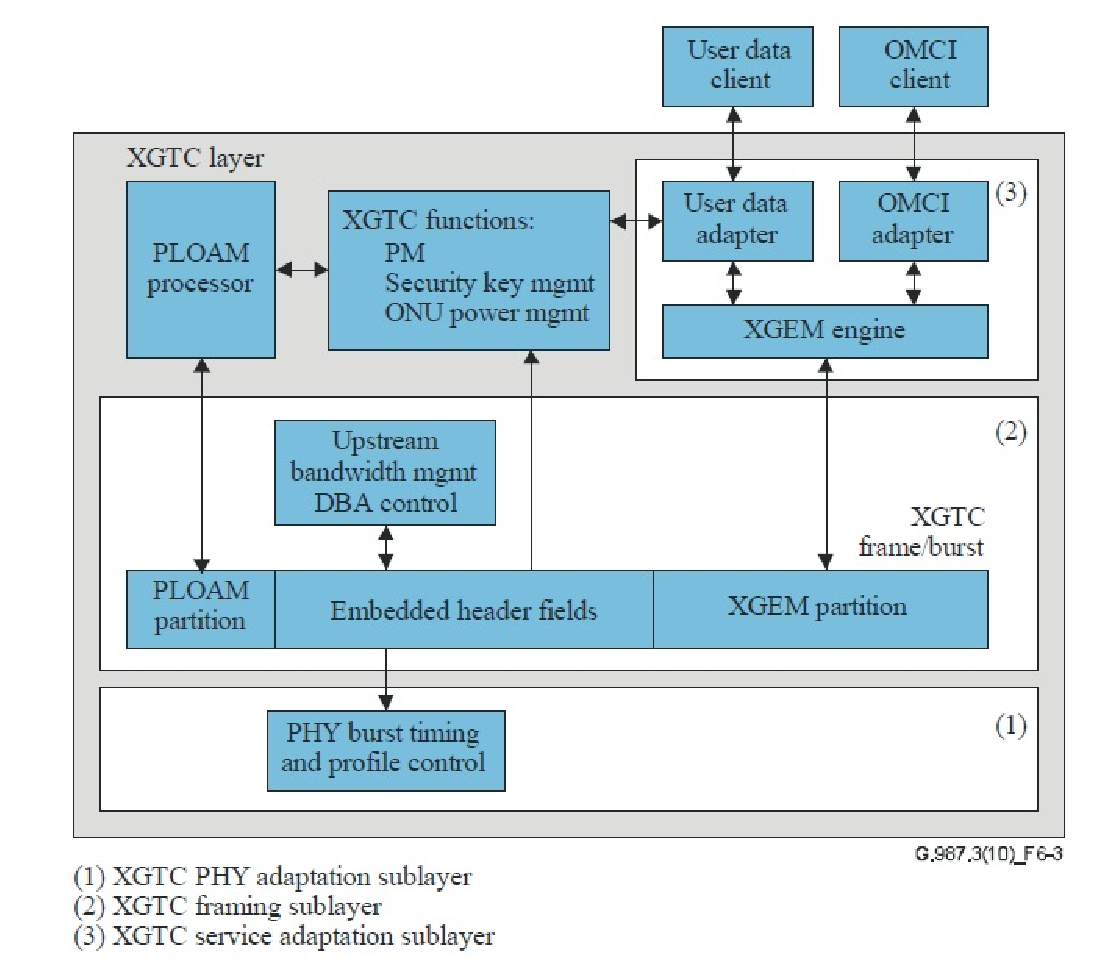
\includegraphics[width=0.75\textwidth]{images/xgtc_infoflow}
\end{center}
\vspace{-0.1in}
\caption{XG-PON Information Flow} \label{figure_xgpon_infoflow}
\end{figure}

\vspace{0.3in}

 \item xgpon-olt-ploam-engine.h/.cc: source code for {\color{red} XgponOltPloamEngine}. XgponOltPloamEngine is one engine
of XgponOltNetDevice. It has a vector of XgponLinkInfo and the index of one XgponLinkInfo equals to the corresponding ONU-ID.
 \item xgpon-onu-ploam-engine.h/.cc: source code for {\color{red} XgponOnuPloamEngine}. XgponOnuPloamEngine is one engine 
of XgponOnuNetDevice. It has one XgponLinkInfo for itself.
\\
{\color{blue} Since our simulation module is designed to study performance issues of one running XG-PON, 
PLOAM messages and the corresponding procedures (activation, ranging, etc.) are not simulated. 
The two classes are used mainly for holding per-ONU information organized within XgponLinkInfo. 
In the future, these classes may be enriched to simulate some PLOAM messages needed by the research.}
\vspace{0.3in}

 \item xgpon-olt-omci-engine.h/.cc: source code for {\color{red} XgponOltOmciEngine}. XgponOltOmciEngine is one engine of XgponOltNetDevice.
 \item xgpon-onu-omci-engine.h/.cc: source code for {\color{red} XgponOnuOmciEngine}. XgponOnuOmciEngine is one engine of XgponOltNetDevice.
\\
{\color{blue} Both the two classes are stub classes. OMCI for XG-PON is very complex and it takes too much time to implement. 
For functions accomplished through OMCI channel (XGEM Port and T-CONT configuration, etc.), we implement through XgponHelper.}
\vspace{0.3in}




 \item xgpon-id-allocator.h/.cc: source code for {\color{red} XgponIdAllocator}. When adding XGEM Port/T-CONT/ONU into XG-PON, 
XgponIdAllocator is used to get one available XGEM Port-Id/Alloc-Id/ONU-ID. There are two subclasses designed for allocating 
these IDs in different ways for different purposes.

 \item xgpon-id-allocator-speed.h/.cc: source code for {\color{red} XgponIdAllocatorSpeed}. As introduced above, 
to speed up XG-PON simulation, we can impose some relationship among XGEM Port-Id, Alloc-Id, ONU-ID, 
and IP address of the node connected to ONU. XgponIdAllocatorSpeed is the subclass designed to impose this relationship.

 \item xgpon-id-allocator-flexible.h/.cc: source code for {\color{red} XgponIdAllocatorFlexible}. 
XgponIdAllocatorFlexible is the subclass of XgponIdAllocator. It does not impose any relationship on XGEM Port-Id, 
Alloc-Id, ONU-ID, and IP address of the node connected to ONU.

 \item xgpon-config-db.h/.cc: source code for {\color{red} XgponConfigDb}. XgponConfigDb is one database 
that holds the information used by XgponHelper to configure XG-PON. For instance, it can be used by the researcher 
to change the subclasses of XgponOltDbaEngine and XgponOltDsScheduler used in the simulation. It also uses 
one flag to make sure that XgponOltConnManagerSpeed, XgponOnuConnManagerSpeed, and XgponIdAllocatorSpeed are used together.

 \item xgpon-helper.h/.cc: source code for {\color{red} XgponHelper}. XgponHelper provides the main interfaces 
needed by researchers for simulating XG-PON. "Install()" is provided to install XgponOltNetDevice on the OLT 
and install XgponOnuNetDevice on all ONUs. In this function, XgponOltNetDevice, XgponOnuNetDevice, and their engines
are created and configured. Thus, before calling "Install()", XgponConfigDb should be used to specify 
the subclasses used in the simulation and the corresponding object factories must be initialized. 
The attributes of some classes (XgponPhy, XgponChannel, etc.) can also be changed before calling "Install()". 
Through XgponHelper, researcher can also enable Ascii or Pcap tracing. In XgponHelper, functions are also 
provided to create XGEM Port and T-CONT for the network. Before calling these functions, XgponHelper 
can be used to change QoS parameters and queue used by XGEM Port.
\\
{\color{blue} This group of files provide the interfaces used by
researchers for simulating XG-PON. Firstly, the researcher need
specify the parameters through XgponConfigDb and XgponHelper.
Secondly, the nodes for the OLT and ONUs must be prepared and
"Install()" of XgponHelper is called to install XponOltNetDevice
and XgponOnuNetDevice on these nodes. Thirdly, after getting the
corresponding IP address of the computers connected to ONUs, XGEM
Port and T-CONT can be configured through XgponHelper. Before
creating XGEM Port or T-CONT, their QoS parameters and queue can
also be changed through XgponHelper.}
\end{enumerate}
